\chapter{Monocular Visual Odometry}\label{chap:initialization}
%In this section, we explain how we implemented our VO pipeline.

Our Visual Odometry pipeline(VO pipeline) consists of initialization, continuous operation, and bundle adjustment as shown in figure \ref{fig:overview}. A loop closure module was also implemented but excluded from the experimental result.

\begin{figure}[h] \label{fig:overview}
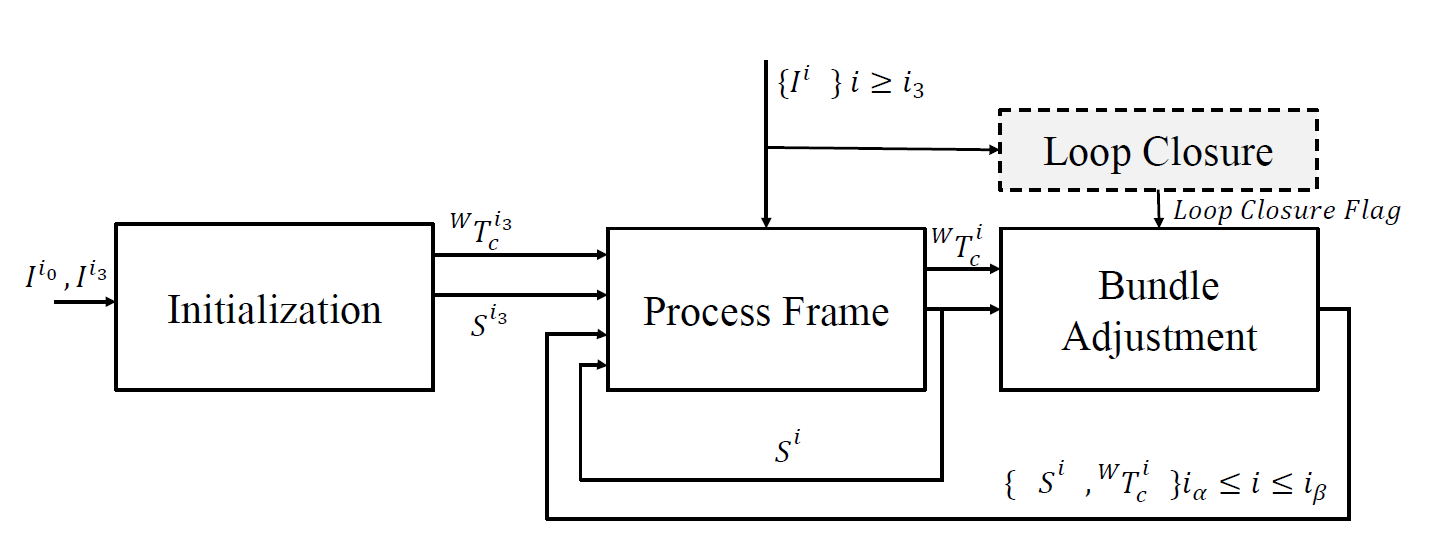
\includegraphics[width=\textwidth]{Overview.png}
\caption{Overview of the visual odometry pipeline.}
\end{figure}

The initialization module outputs the initial pose and landmarks based on the manually selected two images, $I_0$ and $I_1$. The process frame uses the previously estimated pose and landmarks to continuously estimate the current pose. Additionally, VO pipeline performs window-based bundle adjustment to optimize the poses and the landmarks by minimizing the reprojection error in a nonlinear fashion. A loop closure feature was added by storing the landmark history. However, due to the poor robustness of place recognition function, the loop closure feature is not demonstrated properly in the demo videos.

\section{Initialization} \label{sec:initialization}

Our VO pipeline uses a \textbf{monocular standard camera} to estimate initial pose and landmarks. We carefully selected two image frames from each dataset which are sufficiently distant with each other to guarantee stable triangulation performance. 

\subsection*{Initialization for Monocular VO} \label{sec:init_mono}

 Firstly, Harris features are extracted and matched from two selected frames. Based on the matched corners, we apply 8 points RANSAC and obtain a fundamental matrix. The world coordinate frame is the first frame camera pose and the second frame camera pose is calculated by decomposing the fundamental matrix. Additionally, using the inliers from RANSAC, the VO pipepline triangulates new landmarks and removes the landmarks behind the camera. \\
We tested two different error distances for 8 point RANSAC. One is the distance to epipolar line and the other is Sampson error(first-order geometric error). Our VO pipeline uses the distance to epipolar line as both showed qualitatively similar results.

\section{Continuous Operation}\label{sec:continous_operation}
\subsection*{State Propagation}

Our VO pipeline tracks keypoints from previous state using KLT tracker. To cope with the large displacement of keypoints between frames, we use carefully tuned number of pyramids.

\subsection*{Pose Estimation}
The current camera pose is estimated based on the tracked keypoints and their corresponding landmarks. We apply P3P RANSAC to obtain inlier landmarks and initial pose estimation. A nonlinear optimization minimizing the reprojection error was implemented to refine the initial pose estimation. \\
The number of tracked keypoints is constrained to less than a certain number to ensure enough keypoints to estimate the pose of the camera. This saves computational power while estimation.

\subsection*{New Landmarks Triangulation}
Keypoints that are not triangulated are kept as \textbf{candidates} and tracked by KLT tracker. The total number of candidates are constrained by adding a limited number of new candidates in each frame. New candidates are selected among extracted corners that are far enough from existing candidates to avoid selecting certain corners multiple times. 
To check the triangulability of each candidates, we calculate the angle between bearing vectors of the original candidates and the tracked candidates. The angles between the bearing vectors are extremely small, therefore, $\arcsin$ was used instead of $\arctan$ (i.e. \textit{atan2()} function in MATLAB) to take advantage of the numerical stability. Triangulable candidates are updated to new landmarks and used in the pose estimation. 

\section{Bundle Adjustment}
\textbf{A window based optimization strategy} was implemented for a full bundle adjustment. The full bundle adjustment is to prevent drift in pose and landmarks during the continuous operation. The window based optimization strategy deploys a sliding window of $N$ frames for minimizing reprojection error every $M$ frames. Such approach was implemented to reduce the computational complexity while maintaining performance of bundle adjustment. The optimization window $N$ is larger than the bundle adjustment period $N$ so that $N-M$ states overlap with the previous bundle adjustment. \newline
A new data structure, \textbf{bundle adjustment state,} was defined to construct hidden states and observations. After each bundle adjustment, the bundle adjustment state is reconstructed so that the landmark index can be labeled correctly. \newline 
Each dataset is implemented with different sizes of bundle adjustments which shows the best performance for the operating environment. 

\section{Loop Closure}

We tried to implement \textbf{Loop Closure module using place recognition} as follows.

\begin{enumerate}
\item Build a \textbf{bag of visual words} and create \textbf{inverted image index.} Add images which are used for \textit{initialiveVO} step frame to index.
\item For each step of continuous operation, \textbf{retrieve similar images with current image frame} from image index. Check whether retrieved images are from the same place with current place. (Loop detection)
\item If the places are same start loop closure, \textbf{optimize trajectory using bundle adjustment from the beginning to the end of the loop.} Use Harris match for matching landmarks.
\end{enumerate}

The logic to identify the same place is follows.

\begin{itemize}
\item Check if index of retrieved image is distant enough from the current image.
\item Check if the number of retrieved images are enough and their indices are sequential.  
\end{itemize}

The Caltech training set\cite{cvprFei} was used to construct the bag of words but the performance on place recognition on the KITTI or MALAGA dataset images were not sufficient to test the loop closure module. KITTI and MALAGA dataset images were also used to construct the bag of words but the performance of place recognition was not improved. 